\documentclass[slidestop,compress,mathserif]{beamer}
%\documentclass[slidestop,compress,mathserif,handout]{beamer}

%\documentclass[xcolor=dvipsnames,handout]{beamer}
%\documentclass[xcolor=dvipsnames]{beamer}

%\documentclass[handout]{beamer}

%%% To get rid of solutions on hxandouts:
\newcommand{\soln}[1]{\textit{\textcolor{darkGray}{#1}}}				% For slides
%\newcommand{\soln}[1]{ }	% For handouts

% to get pausing to work properly on slides
\newcommand{\hide}[1]{#1}	% For slides
%\newcommand{\hide}[1]{ }	% For handouts


%\usepackage{multicol}
\usepackage{amsfonts}
%\usepackage[pdftex,dvipsnames]{color}
\usepackage{graphicx}
\usepackage{subfigure}
%\usepackage{picinpar}
\usepackage{pifont}
\usepackage{pgf,pgfarrows,pgfnodes}
%\usepackage{wasysym,manfnt,phaistos,empheq}
\usepackage[english]{babel}
\usepackage{pgfpages}
\usepackage{natbib}
\usepackage{hyperref}
\usepackage{multimedia}
%\usepackage{amsfonts,amstext,amssymb,amsbsy,amsopn,amsthm,eucal,latexsym,mathrsfs}
\usepackage{amsmath,amsfonts,amstext,amssymb,amsbsy,amsopn,amsthm,eucal,latexsym,mathrsfs}
\usepackage{ulem}
\usepackage{setspace}
\usepackage{array}
%\usepackage{rotating}
\usepackage{multirow}
\usepackage{verbatim}
\usepackage{multicol}

\setbeamertemplate{navigation symbols}{}

%\usepackage{tikz}
%\usetikzlibrary{arrows,shapes,trees,backgrounds}


%\setbeameroption{show notes on second screen}
%\setbeameroption{show notes}
%\setbeameroption{show only notes}

\definecolor{links}{HTML}{2A1B81}
\hypersetup{colorlinks,linkcolor=,urlcolor=links}

\newtheorem*{principle}{Inscrutibility Principle}
\newtheorem*{punchline}{Punch Line}
\newtheorem{defn}{Definition}

\definecolor{Scarlet}{RGB}{140,17,17}
\definecolor{VassarRed}{RGB}{128,0,0}

% "dinglist" environment
  \renewenvironment{dinglist}[2][blue]
  {\begin{list}{\textcolor{blue}{\ding{#2}}}{}}{\end{list}}
  % Symbol definitions for these lists
  \newcommand{\DingListSymbolA}{43}
  \newcommand{\DingListSymbolB}{243}
  \newcommand{\DingListSymbolC}{224}
  \newcommand{\DingListSymbolD}{219}
  \newcommand{\DingListSymbolCheck}{52}
  \newcommand{\DingListSymbolCross}{56}


  \newenvironment{ballotenv}
{\only{%
\setbeamertemplate{itemize item}{\ding{45}}%
\setbeamertemplate{itemize subitem}{\ding{46}}%
\setbeamertemplate{itemize subsubitem}{\ding{46}}}} {}
\setbeamertemplate{itemize item}{\ding{49}}
\setbeamertemplate{itemize subitem}{\ding{47}}
\setbeamertemplate{itemize subsubitem}{\ding{47}}


%User defined colors: See colors section
\xdefinecolor{oiBlue}{rgb}{0.15, 0.35, 0.55}
\xdefinecolor{gray}{rgb}{0.5, 0.5, 0.5}
\xdefinecolor{darkGray}{rgb}{0.3, 0.3, 0.3}
\xdefinecolor{darkerGray}{rgb}{0.2, 0.2, 0.2}
\xdefinecolor{rubineRed}{rgb}{0.89,0,0.30}
\xdefinecolor{linkCol}{rgb}{0.11,0.49,0.95}	
\xdefinecolor{irishGreen}{rgb}{0,0.60,0}	
\xdefinecolor{darkturquoise}{rgb}{0.44, 0.58, 0.86}
\definecolor{lightGreen}{rgb}{0.533,0.765,0.42}
\xdefinecolor{Regalia}{HTML}{522D80}
\xdefinecolor{ClemsonOrange}{HTML}{EA6A20}

\definecolor{duke@LightGrey}{RGB}{200,200,200}\definecolor{DarkGreen}{RGB}{0,100,0}
\definecolor{Oranges}{RGB}{255,127,0}
\definecolor{LightGray}{RGB}{211,211,211}

%\setbeamertemplate{footline}{%
%  \raisebox{5pt}{\makebox[\paperwidth]{\hfill\makebox[10pt]{\scriptsize\insertframenumber}}}}

\setbeamercolor{equation background}{fg=black,bg=duke@LightGrey}
  % Boxed equation
  \newcommand{\eqbox}[2][0.6]{%
  \centerline{
  \begin{beamerboxesrounded}[lower=equation background,width=#1\hsize,shadow=true]{}
\parbox{#1\hsize}{%
      \[
        \textcolor{black} {#2}
      \]}
  \end{beamerboxesrounded}
}}

\AtBeginSection[] {
  \begin{frame}<beamer>\frametitle{Outline}
    \tableofcontents[currentsection,hideothersubsections]
  \end{frame}
}
%
%
%\AtBeginSubsection[] {
%  \begin{frame}<beamer>\frametitle{Outline}
%    \tableofcontents%[currentsection,currentsubsection]
%  \end{frame}
%}

%\usecolortheme[RGB={82,45,128}]{structure}
%\usecolortheme[RGB={162,80,22}]{structure}
\usecolortheme[RGB={128,0,0}]{structure}
\usetheme[secheader]{Boadilla}
%\usetheme[height=7mm]{Rochester}
%\usetheme{Copenhagen}
%\usetheme{Antibes}
%\usecolortheme{seahorse}
%\usecolortheme{crane}
%\usecolortheme{rose}
%\usefonttheme[onlylarge]{structurebold}
%\usefonttheme[onlymath]{serif}



\def\diag{{\rm diag}}


\def\E{\mathbb{E}}
\def\Prob{\mathbb{P}}
\def\argmin{{\rm argmin}}
\def\argmax{{\rm argmax}}
\def\Def{\stackrel{def}{=}}


\newtheorem{assumption}{Assumptions}
\newtheorem*{proposition}{Proposition}
\newtheorem*{remark}{Remark}



%\setbeamercolor{disc title}{bg=oiBlue!40!white!60,fg=blue}
\setbeamercolor{disc body}{bg= Regalia!20!white!80,fg= Regalia!80!black!90}

\setbeamercolor{clicker ungraded title}{bg=irishGreen!80!white!50,fg=irishGreen!30!black!90}
\setbeamercolor{clicker ungraded body}{bg=irishGreen!20!white!80,fg=irishGreen!30!black!90}

\setbeamercolor{clicker review title}{bg=gray!80!white!80,fg=oiBlue!80!black!90}
\setbeamercolor{clicker review body}{bg=gray!30!white!90,fg=oiBlue!80!black!90}

\setbeamercolor{code body}{bg=gray!20!white!80,fg=black}


% Custom commands
\newcommand{\degree}{\ensuremath{^\circ}}
\newcommand{\Note}[1]{
\rule{2.5cm}{0.25pt} \\ \textit{\scriptsize {\textcolor{rubineRed}{Note:} \textcolor{gray}{#1}}}}
\newcommand{\ct}[1]{
\vfill
{\tiny #1}}
\newcommand{\Remember}[1]{\textit{\scriptsize{\textcolor{orange}{Remember:} \textcolor{gray}{#1}}}}
\newcommand{\red}[1]{\textit{\textcolor{rubineRed}{#1}}}
\newcommand{\pink}[1]{\textit{\textcolor{rubineRed!90!white!50}{#1}}}
\newcommand{\green}[1]{\textit{\textcolor{irishGreen}{#1}}}
\newcommand{\webURL}[1]{\urlstyle{same}\textit{\textcolor{linkCol}{\url{#1}}} }
\newcommand{\webLink}[2]{\href{#1}{\textcolor{linkCol}{{#2}}}}
\newcommand{\mail}[1]{\href{mailto:#1}{\textit{\textcolor{linkCol}{#1}}}}
\newcommand{\hl}[1]{\textit{\textcolor{oiBlue}{#1}}}
\newcommand{\hlGr}[1]{\textit{\textcolor{lightGreen}{#1}}}
\newcommand{\mathhl}[1]{\textcolor{oiBlue}{\ensuremath{#1}}}
\newcommand{\ex}[1]{\textcolor{blue}{{{\small (#1)}}}}
\newcommand{\disc}[1]{
\begin{beamerboxesrounded}[shadow = true, lower = disc body, upper = disc title]{}
#1
\end{beamerboxesrounded}
}

\newcommand{\cl}[1]{
\begin{beamerboxesrounded}[shadow = true, lower = clicker ungraded body, upper = clicker ungraded title]{Question}
$\:$ \\
#1
\end{beamerboxesrounded}
}

\newcommand{\clR}[1]{
\begin{beamerboxesrounded}[shadow = true, lower = clicker review body, upper = clicker review title]{\red{Review question} }
$\:$ \\
#1
\end{beamerboxesrounded}
}

\newcommand{\formula}[2]{
\begin{beamerboxesrounded}[shadow = true, lower = white, upper = clicker review body]{#1}
#2
\end{beamerboxesrounded}
$\:$ \\
}

\newenvironment{twocol}[4]{
\begin{columns}[c]
\column{#1\textwidth}
#3
\column{#2\textwidth}
#4
\end{columns}
}


\newenvironment{slot}[2]{
\begin{array}{c}
\underline{#1} \\
#2
\end{array}
}

\newcommand{\pr}[1]{
\left( #1 \right)
}

\newcommand{\solnMult}[1]{
\item[] \vspace{-0.59cm}
\only<beamer| beamer:1>{\item #1}
\soln{\only<2->{\item \red{#1}}}
}

%\newcommand{\codechunk}[1]{
%\begin{beamerboxesrounded}[shadow = true, lower = code body]{}
%{\small #1}
%\end{beamerboxesrounded}
%}

% Change margin

\newenvironment{changemargin}[2]{%
\begin{list}{}{%
\setlength{\topsep}{0pt}%
\setlength{\leftmargin}{#1}%
\setlength{\rightmargin}{#2}%
\setlength{\listparindent}{\parindent}%
\setlength{\itemindent}{\parindent}%
\setlength{\parsep}{\parskip}%
}%
\item[]}{\end{list}}

% Footnote

\long\def\symbolfootnote[#1]#2{\begingroup%
\def\thefootnote{\fnsymbol{footnote}}\footnote[#1]{#2}\endgroup}

% Commands from the book
\newenvironment{data}[1]{\texttt{#1}}{}
\newenvironment{var}[1]{\texttt{#1}}{}
\newenvironment{resp}[1]{\texttt{#1}}{}






%%%%%%%%%%%%%%%%%%%%%%%%%%%%%%%%%%%%%%%%%%%%%%%%%%%%%%%%%%%%%%%%%%%%%%%%%%%%%%%%%%%%%%%%%%%%%%%

\title[Chapter 4 part 3]{Chapter 4 part 3}
\subtitle{Discrete Random Variables}

%%%%%%%%%%%%%%%%%%%%%%%%%%%%%%%%%%%%%%%%%%%%%%%%%%%%%%%%%%%%%%%%%%%%%%%%%%%%%%%%%%%%%%%%%%%%%%%


\author[Jingchen (Monika) Hu] % (optional, use only with lots of authors)
{Jingchen (Monika) Hu}
% - Give the names in the same order as the appear in the paper.
% - Use the \inst{?} command only if the authors have different
%   affiliation.

\institute[Vassar] % (optional, but mostly needed)
{Vassar College}
% - Use the \inst command only if there are several affiliations.
% - Keep it simple, no one is interested in your street address.

\date[MATH 241] % (optional, should be abbreviation of conference name)
{MATH 241}
% - Either use conference name or its abbreviation.
% - Not really informative to the audience, more for people (including
%   yourself) who are reading the slides online

\subject{MATH 241}
% This is only inserted into the PDF information catalog. Can be left
% out.



% If you wish to uncover everything in a step-wise fashion, uncomment
% the following command:

%\beamerdefaultoverlayspecification{<+->}


\begin{document}




%%%%%%%%%%%%%%%%%%%%%

% Title Page

\begin{frame}%[plain]
\titlepage
\end{frame}

%%%%%%%%%%%%%%%%%%%%%
%\addtocounter{framenumber}{-1}
%
%\begin{frame}\frametitle{Annoucement}
%
%\begin{itemize}
%\item HW3: \red{due now!}
%\item HW4: \red{due Tuesday, Sept 30th}
%\end{itemize}
%
%
%\end{frame}
%
%





%%%%%%%%%%%%%%%%%%%%%%%%%%%%%%%%%%%%%%%%%%
\section{Poisson distribution}
%%%%%%%%%%%%%%%%%%%%%%%%%%%%%%%%%%%%%%%%%%
\addtocounter{framenumber}{-1}
\begin{frame}\frametitle{Count the number of ...}

\twocol{0.25}{0.75}{
\begin{center}

\includegraphics[width = \textwidth]{figures/guinness}
\end{center}
\uncover<2>{
\begin{center}

\includegraphics[width = 0.7\textwidth]{figures/prussian_soldier}
\end{center}
}
}
{
In beer brewing, cultures of yeast are kept alive in jars of fluid before being put into the mash.
\begin{itemize}
\item It's critical to control the amount of yeast used. %in the mash:
%too little leads to incomplete fermentation; to much leads to bitter beer.
\item Number of yeast cells in a fluid sample can be seen under a microscopes.
\item Yeast cells are constantly multiplying and dividing.
\item A famous statistician, Wiliam Sealy Gosset (aka ``Student''), who worked
for the Guinness Brewing Compnay in early 1900's, modeled
the counts of yeast cells using the \red{Poisson distribution}.
\end{itemize}

\uncover<2>{
\vspace{24pt}
The Poisson distribution was used in 1898 to count the number of
soldiers in the Prussian Army
who died accidentally from horse kicks

}
}

\end{frame}

%%%%%%%%%%%%%%%%%%%%%%%%%%%%%%%%%%%%%%%%%%
\begin{frame}\frametitle{Poisson distribution}
\begin{defn}%{\DingListSymbolA}
Denote random variable $X$ that takes value in $\{0, 1, 2, \ldots\}$ as having a \hl{Poisson distribution}
 with parameter $\lambda$ if its pmf is
\[ X \sim \text{P}(\lambda) \Longleftrightarrow\ p(k) = e^{-\lambda}\ \frac{\lambda^k}{k!},\quad k = 0, 1, 2, \ldots \]
\end{defn}

\pause
\twocol{0.75}{0.25}{
\begin{itemize}
\item Formulated by French mathematician\\ Sim\'{e}on Denis Poisson
\pause
\item Usually is used to model "the number of xxx occur". Hence lower bound is $0$, no upper bound.
\pause
\item Examples
\begin{itemize}
\item Number of rainy days this year
\pause
\item Number of mis-placed books in the Main library
%\item Number of times the song ``just give me a reason'' played in FM102.5
\pause
\item Number of roses you will receive on the next Valentines Day
\end{itemize}

\end{itemize}
}
{
\pause
\begin{center}
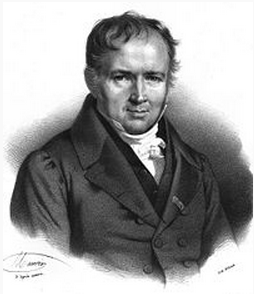
\includegraphics[width = \textwidth]{figures/Simeon_Denis_Poisson}
\end{center}
}

\end{frame}



%%%%%%%%%%%%%%%%%%%%%%%%%%%%%%%%%%%%%%%%%%
\begin{frame}\frametitle{Pmf of Poisson distribution}

\vspace{-0.5cm}
\begin{center}
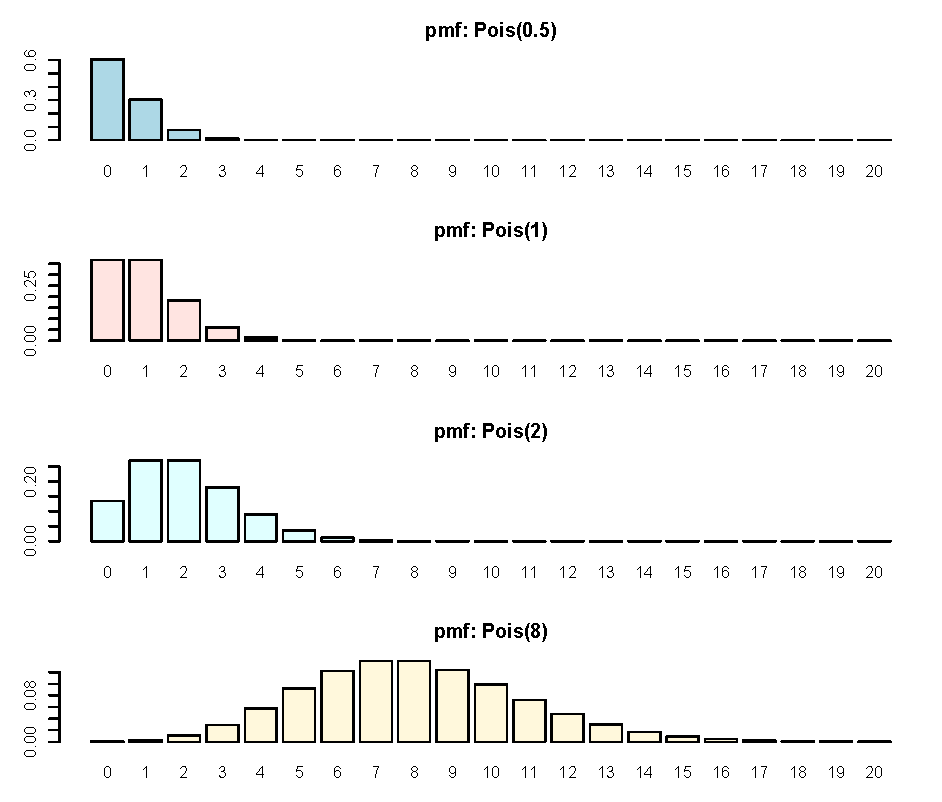
\includegraphics[scale = 0.6]{figures/pmf3}
\end{center}

\end{frame}

%%%%%%%%%%%%%%%%%%%%%%%%%%%%%%%%%%%%%%
%
%\begin{frame}\frametitle{Mode of Poisson distribution}
%
%\begin{itemize}
%\item $X \sim \text{P}(\lambda)$. Then as $k$ goes from $0$ to $\infty$,
%\begin{align*}
%& p(k) \text{ increases  for } 0 \leq k \leq \lambda - 1\\
%& p(k) \text{ decreases   for }  k > \lambda -1
%\end{align*}
%\end{itemize}
%\red{Proof}
%
%%\invisible{
%\pause
%\[
%\frac{p(k + 1)}{p(k)} = \frac{ e^{-\lambda}\ \frac{\lambda^{k+1}}{(k+1)!} }{ e^{-\lambda}\ \frac{\lambda^k}{k!} }
%= \frac{\lambda}{k + 1}
%\]
%\[
%p(k) \text{ increases} \Longleftrightarrow \frac{p(k + 1)}{p(k)} \geq 1 \Longleftrightarrow k \leq \lambda -1
%\]
%
%%}
%
%\end{frame}
%
%%%%%%%%%%%%%%%%%%%%%%%%%%%%%%%%%%%%%%%%%%
\begin{frame}\frametitle{Properties of Poisson distribution $p(k) = e^{-\lambda}\ \frac{\lambda^k}{k!}$}

\begin{itemize}
\item Well-defined (validness of pmf): non-negative, and
\[\sum_{k = 0}^{\infty} p(k) = 1\]
\end{itemize}

\vfill
\begin{itemize}
\item Taylor Series
\[ f(x) = f(x_0) + \frac{x-x_0}{1!}f^{\prime}(x_0) + \frac{(x-x_0)^2}{2!} f^{\prime\prime}(x_0) + \cdots \]

\item Use Taylor series to verify that the Poisson distribution is well-defined  ({\color{red}required})
\[ e^{\lambda} = 1 + \lambda + \frac{\lambda^2}{2!} + \cdots + \frac{\lambda^k}{k!}+\cdots\]
\end{itemize}



\end{frame}
%%%%%%%%%%%%%%%%%%%%%%%%%%%%%%%%%%%%%%%%%%
\begin{frame}\frametitle{Properties of Poisson distribution $p(k) = e^{-\lambda}\ \frac{\lambda^k}{k!}$}

\begin{itemize}
\item Mean ({\color{red}required}) textbook page 137
\[E[X] = \lambda \]

\vspace{15mm}
\pause
\item Variance ({\color{red}required}) textbook page 138
\[Var[X] = \lambda \]

\end{itemize}

\end{frame}


%%%%%%%%%%%%%%%%%%%%%%%%%%%%%%%%%%%%%%%%%%
\begin{frame}%\frametitle{Pmf of Binomial distribution: uni-modeal}
\disc{Suppose Vassar students have 1.73 siblings on average.
What's the probability that a randomly selected student has at most one sibling?
}

%\twocol{0.2}{0.8}{
%\begin{enumerate}[(a)]
%\item $0.5$
%\item $1/e$
%\solnMult{$2/e$}
%\item $1 - 1/e$
%\end{enumerate}
%}
{
%\invisible{
\pause\vspace{0.5cm}

\[ X \sim \text{P}(\lambda), E[X] = 1.73 \Longrightarrow \lambda = 1.73 \]
\begin{align*}
P(X \leq 1) &= p(0) + p(1)\\
& = e^{-\lambda} \frac{\lambda^0}{0!} +  e^{-\lambda} \frac{\lambda^1}{1!}\\
& = 0.1773 + 0.3067 = 0.4840
\end{align*}
%}
}

\end{frame}

%%%%%%%%%%%%%%%%%%%%%%%%%%%%%%%%%%%%%%%%%%
\begin{frame}\frametitle{Use Poisson to approximate Binomial distribution} % for small $p$ and large $n$}

Let $X \sim \text{Bin}(n, p)$. If
\begin{itemize}
\item $p$: small
\item $n$: large
\item $\lambda = np$: of moderate size
\end{itemize}
then the distribution of $X$ can be approximated by $\text{P}(\lambda)$.\\
\pause
\begin{center}
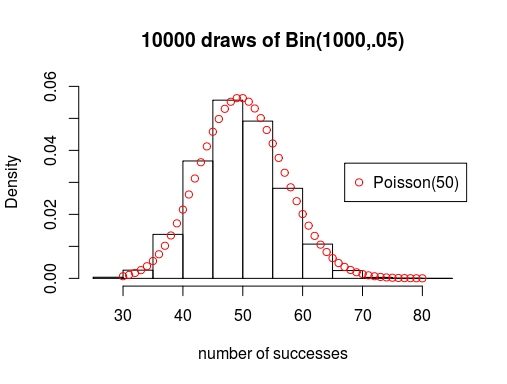
\includegraphics[width = 0.5\textwidth]{figures/poisson_approx_binom}
\end{center}
%\red{Proof}

\end{frame}

%%%%%%%%%%%%%%%%%%%%%%%%%%%%%%%%%%%%%%%%%%
\begin{frame}\frametitle{Recap}

Poisson distribution $X \sim \text{P}(\lambda) $
\[ p(k) = e^{-\lambda}\ \frac{\lambda^k}{k!}\]
\begin{itemize}
\item mean $\mu = \lambda$
\item variance $\sigma^2 =  \lambda$
\item Approximate Binomial distribution with small $p$, large $n$, moderate $np$
\[ \text{P}(np) \approx \text{Bin}(n,p) \]
%\item Poisson process PP$(\lambda)$
%\[ N(t) \sim \text{P}(\lambda t) \]
\end{itemize}


\end{frame}



%%%%%%%%%%%%%%%%%%%%%%%%%%%%%%%%%%%%%%%%%%
\section{Geometric distribution and Negative Binomial distribution}
%%%%%%%%%%%%%%%%%%%%%%%%%%%%%%%%%%%%%%%%%%

\begin{frame}\frametitle{Geometric distribution}

A gambler plays at a roulette table and alway bet on red until he wins...\\
In each round, his chance of winning is $18/38 = 0.47$.\\
Let $X$ denote the number of rounds he plays.

\pause
\begin{defn}
Denote random variable $X$ that takes value in $\{1, 2, \ldots\}$ as having a \hl{Geometric distribution}
 with parameter $p \in (0, 1)$ if its pmf is
\[ X \sim \text{Geometric}(p) \Longleftrightarrow\ p(k) = (1-p)^{k-1}p,\quad k = 1, 2, \ldots \]
\end{defn}
\pause
\begin{itemize}
\item $X$ represents the number of trials performed until we get a success, where $p$ is the probability of success on each trial.
\pause
\item Note the difference between Geometric distribution and Binomial distribution!
\pause Eg: whether the total number of trials is fixed.
\end{itemize}

\end{frame}

%%%%%%%%%%%%%%%%%%%%%%%%%%%%%%%%%%%%%%%%%%
\begin{frame}\frametitle{Properties of Geometric distribution $p(k) = (1-p)^{k-1}p$}

\begin{itemize}
\item Well-defined (validness of pmf): non-negative, $\sum_{k = 1}^{\infty} p(k) = 1$  ({\color{red}required})\\
%\invisible{
\pause\vspace{-0.3cm}
\[\sum_{k = 1}^{\infty}(1-p)^{k-1}p =  p[1 + (1-p) + (1-p)^2 + \cdots] = \frac{p}{1-(1-p)}=1 \]
%}

\vspace{0.5cm}
\pause
\item Cdf: $P(X \leq k) = 1 - (1-p)^k$  ({\color{red}required})\\
%\invisible{
\pause\vspace{-0.3cm}
\[ P(X \geq k + 1) = P(\text{The first } k \text{ trials all fail}) \]
%}

\pause\item Mean ({\color{red}not required}) Textbook page 148 for derivation
\[E[X] = \frac{1}{p} \]

\pause\item Variance ({\color{red} not required}) Textbook page 148 for derivation
\[Var[X] = \frac{1-p}{p^2} \]
\end{itemize}

\end{frame}


%%%%%%%%%%%%%%%%%%%%%%%%%%%%%%%%%%%%%%%%%%
\begin{frame}\frametitle{Gambler's fallacy}
If the gambler loses 5 times in a row, will he more likely to win in the 6th round?
\pause
\[
P(X > 6 \mid X > 5) \stackrel{?}{<} P(X > 1)
\]
\pause
Unfortunately, not.
\pause
\begin{defn}
We say a distribution is \hl{memoryless}, if
\[ P(X > n + k \mid X > n) = P(X > k)\]
\end{defn}

\pause
\begin{itemize}
\item Geometric random variable is memoryless.

%\invisible{
\pause
%Let $q = (1-p)$, then
\begin{align*}
P(X > n + k \mid X > n) %& = \frac{P(X > n + k \cap X > n)}{P(X > n)} \\
& = \frac{P(X > n + k)}{P(X > n)} \\
%& =  \frac{P(\text{first } n + k \text{ trials all fail})}{P(\text{first } n \text{ trials all fail})} \\
& = \frac{(1-p)^{n+k}}{(1-p)^n} = (1-p)^k = P(X > k)
\end{align*}
%}

\end{itemize}

\end{frame}

%%%%%%%%%%%%%%%%%%%%%%%%%%%%%%%%%%%%%%%%%%
\begin{frame}\frametitle{Pmf of Geometric distribution}

\vspace{-0.5cm}
\begin{center}
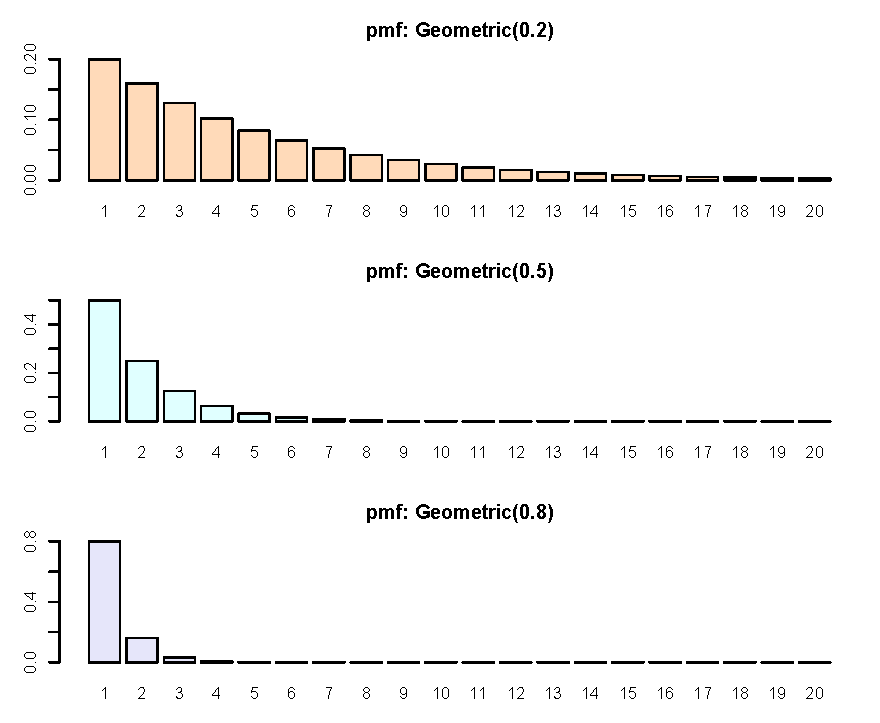
\includegraphics[scale = 0.63]{figures/pmf4}
\end{center}

\end{frame}


%%%%%%%%%%%%%%%%%%%%%%%%%%%%%%%%%%%%%%%%%%
\begin{frame}\frametitle{Negative Binomial distribution}
\begin{defn}
Denote random variable $X$ that takes value in $\{1, 2, \ldots\}$ as having a \hl{Negative Binomial distribution}
 with parameter $p \in (0, 1)$ if its pmf is
\[ X \sim \text{NB}(r, p) \Longleftrightarrow\ p(k) = {k - 1 \choose r - 1}(1-p)^{k-r}p^{r},\quad k = r, r+1, \ldots \]
\end{defn}

\begin{itemize}
\item $X$ represents the number of trials performed until we get $r$ success, where $p$ is the probability of success on each trial.

\pause
\item Well-defined (validness of pmf). ({\color{red}not required})


\pause
\item Connection between Negative Binomial and Geometric distributions
\[ X \sim \text{Geometric}(p) \Longleftrightarrow  X \sim \text{NB}(1, p) \]


\end{itemize}

\Note{Proof of $\sum_{k = r}^{\infty} p(k) = 1$ for Negative Binomial distribution is not required.}

\end{frame}

%%%%%%%%%%%%%%%%%%%%%%%%%%%%%%%%%%%%%%%%%%
\begin{frame}\frametitle{Properties of Neg Binom $p(k) = {k - 1 \choose r - 1}(1-p)^{k-r}p^{r}$}

\vfill
\begin{itemize}
\item Mean ({\color{red}not required})
\[E[X] = \frac{r}{p} \]
Textbook page 150 for derivation
\pause
\item Variance ({\color{red}not required})
\[Var[X] = \frac{r(1-p)}{p^2} \]
Textbook page 151 for derivation
\pause
\item Recall that for $\text{Geometric}(p)$,
\[ \mu = \frac{1}{p}, \sigma^2 = \frac{1-p}{p^2}\]
%\red{Proof}


\end{itemize}

\end{frame}



%%%%%%%%%%%%%%%%%%%%%%%%%%%%%%%%%%%%%%%%%%
\begin{frame}\frametitle{Pmf of Negative Binomial distribution}

\vspace{-0.5cm}
\begin{center}
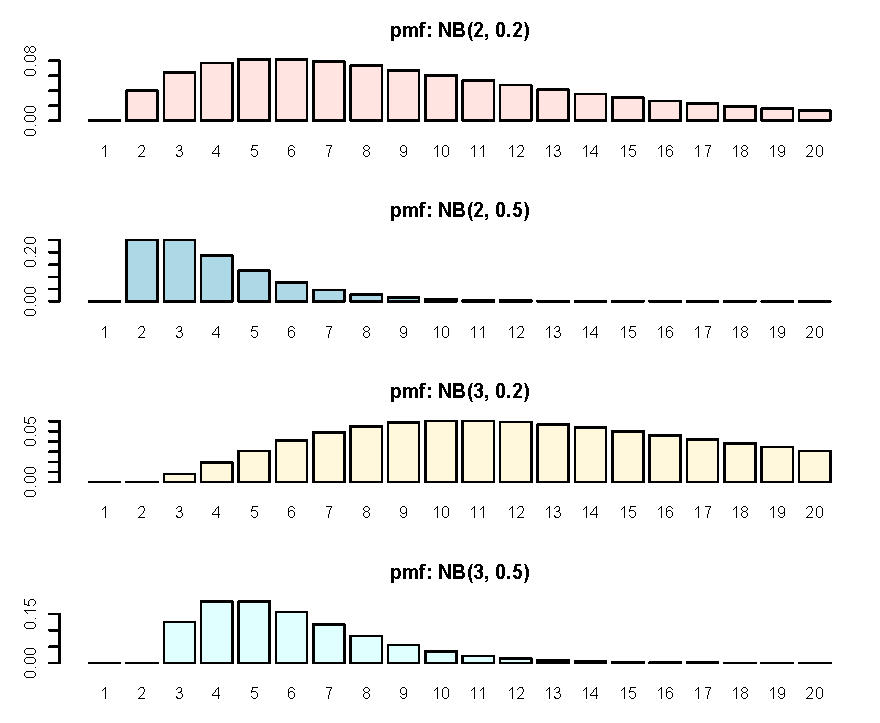
\includegraphics[scale = 0.63]{figures/pmf5}
\end{center}

\end{frame}


%%%%%%%%%%%%%%%%%%%%%%%%%%%%%%%%%%%%%%%%%%



%%%%%%%%%%%%%%%%%%%%%%%%%%%%%%%%%%%%%%%%%%
\begin{frame}\frametitle{Recap}

$X$: the number of trials performed until we get $r$ success, where $p$ is the probability of success on each trial.
\[ p(k) = {k - 1 \choose r - 1}(1-p)^{k-r}p^{r},\quad k = r, r+1, \ldots \]
\vspace{-0.5cm}
\begin{itemize}
\item Negative Binomial distribution $X \sim \text{NB}(r, p)$
\item Mean $\mu = \frac{r}{p}$, variance $\sigma^2 = \frac{r(1-p)}{p^2}$.
\item If $r = 1$, Geometric distribution $X \sim \text{NB}(1, p) = \text{Geometric}(p)$
\item Geometric distribution is memoryless.
\end{itemize}

%\vspace{0.5cm}\pause
%$X$: the number of white balls selected among $n$ balls from a box containing
%$m$ whites balls and $N-m$ black balls.
%\begin{itemize}
%\item Hypergeometric distribution $X \sim \text{HG}(n, N, m)$.
%\item Mean $\mu = \frac{nm}{N}$ %, variance $\sigma^2 = \frac{r(1-p)}{p^2}$.
%\end{itemize}


\end{frame}

%%%%%%%%%%%%%%%%%%%%%%%%%%%%%%%%%%%%%%%%%%
\begin{frame}\frametitle{Review: discrete distributions}

\begin{center}
\begin{tabular}{lllcc}
\hline
Name 								& Range 			& pmf $p(x)$																& mean 						& variance \\
\hline
Ber$(p)$							& $\{0, 1\}$			& $p^x (1-p)^{1-x}$														& $p$						& $p(1-p)$\\
&&&&\\
\uncover<2->{Bin$(n, p)$				& $\{0, 1, \ldots, n\}$	& ${n \choose x} p^x (1-p)^{n-x}$											& $np$						& $np(1-p)$\\}
&&&&\\
\uncover<3->{Pois$(\lambda)$		& $\{0, 1, 2, \ldots\}$	& $e^{-\lambda}\ \frac{\lambda^x}{x!}$										& $\lambda$				& $\lambda$\\}
&&&&\\
\uncover<4->{Geometric$(p)$		& $\{1, 2, \ldots\}$	& $(1-p)^{x-1}p$															& $\frac{1}{p}$				& $\frac{1-p}{p^2}$\\}
&&&&\\
\uncover<5->{NegBin$(r, p)$			& $\{r, r+1, \ldots\}$	& ${x - 1 \choose r - 1}(1-p)^{x-r}p^{r}$									& $\frac{r}{p}$				& $\frac{r(1-p)}{p^2}$\\ \hline}
&&&&\\
%\uncover<6->{HG$(n, N, m)$			& $\{0, 1, \ldots, n\}$	& $\frac{ {m \choose x}{N - m \choose n - x} }{ {N \choose n} }$				& $\frac{mn}{N} $			& $ \frac{N-n}{N-1} \frac{nm(N-m)}{N^2}$\\
%\hline}
\end{tabular}
\end{center}

\end{frame}





\end{document} 